%%%%%%%%%%%%%%%%%%%%%%%%%%%%%%%%%%%%%%%%%%%%%%%%%%%%%%%%%%%%%%%%%%%%%%%%
\clearpage
\section{Plugin functions for SESANS}
\label{ch:pluginsSESANS}

The depolarization of the neutron beam as a function of the spin-echo length $z$ is given by
\begin{align}
\frac{P_n(z)}{P_{n0}}&=\exp\left(\mathcal{G}(z)-\mathcal{G}(0)\right)
\end{align}
where the unnormalized SESANS correlation function reads as
\begin{align}
\mathcal{G}(z) &= \frac{1}{k_0^2} \int_{-\infty}^{\infty}\int_{-\infty}^{\infty} \mathrm{d}Q_y\, \mathrm{d}Q_z \frac{\mathrm{d}\Sigma(\mathbf{Q})}{\mathrm{d}\Omega}\frac{\cos(Q_z z)}{S} \\
             &= \frac{1}{k_0^2} \int_{-\infty}^{\infty}\int_{-\infty}^{\infty} \mathrm{d}Q_y\, \mathrm{d}Q_z  \frac{\mathrm{d}\sigma(\mathbf{Q})}{\mathrm{d}\Omega}t \cos(Q_z z)
\end{align}
with $\mathbf{Q}=(0,Q_y,Q_z)^T$ and $\frac{\mathrm{d}\Sigma(\mathbf{Q})}{\mathrm{d}\Omega}$ being the macroscopic differential scattering cross-section in units of cm$^2$ and $\frac{\mathrm{d}\sigma(\mathbf{Q})}{\mathrm{d}\Omega}=\frac{1}{V}\frac{\mathrm{d}\Sigma(\mathbf{Q})}{\mathrm{d}\Omega}$ the differential scattering cross-section normalized on the sample volume $V=tS$ in units of cm$^{-1}$. $t$ is the sample thickness and $S$ the aperture cross-section defining the illuminated sample area. For isotropic scattering $\frac{\mathrm{d}\sigma(\mathbf{Q})}{\mathrm{d}\Omega}=\frac{\mathrm{d}\sigma(Q)}{\mathrm{d}\Omega}$, where the scattering only depends on the modulus of the scattering vector $Q=\abs{\mathbf{Q}}$ the unnormalized SESANS correlation function simplifies to a Hankel transform of the scattering intensity multiplied by $\frac{\lambda^2 t}{2\pi}$. To see this, one has to change from cartesian coordinates $(0,Q_y,Q_z)$ to polar coordinates $Q (0,\sin\phi,\cos\phi)$ with $\mathrm{d}Q_y \mathrm{d}Q_z = Q\mathrm{d}Q \mathrm{d}\phi$. The integration over $\phi$ yield the cylindrical zeroth-order Bessel function
\begin{align}
J_0(Qz)=\frac{1}{2\pi}\int_{0}^{2\pi} \cos\left(Q\cos(\phi)z\right) \mathrm{d}\phi
\end{align}
so that one gets
\begin{align}
\mathcal{G}(z) &= \frac{2\pi t}{k_0^2} \int_{0}^{\infty} Q J_0(Qz) \frac{\mathrm{d}\sigma(Q)}{\mathrm{d}\Omega} \, \mathrm{d}Q \\
&= \frac{\lambda^2 t}{4\pi^2} 2\pi\underbrace{\int_{0}^{\infty} Q J_0(Qz) \frac{\mathrm{d}\sigma(Q)}{\mathrm{d}\Omega} \, \mathrm{d}Q}_{\mathcal{H}_0\left\{\frac{\mathrm{d}\sigma(Q)}{\mathrm{d}\Omega}\right\}} = \frac{\lambda^2 t}{4\pi^2}  2\pi \mathcal{H}_0\left\{\frac{\mathrm{d}\sigma(Q)}{\mathrm{d}\Omega}\right\} = \frac{\lambda^2 t}{4\pi^2} \tilde{G}(z)
\end{align}
where $\tilde{G}(z)=2\pi\mathcal{H}_0\left\{\frac{\mathrm{d}\sigma(Q)}{\mathrm{d}\Omega}\right\}$ and $\mathcal{H}_0\left\{\ldots\right\}$ denotes the Hankel transform of zeroth order.\footnote{
There are several possible definitions of a Hankel transform $\mathcal{H}_\nu\left\{f(r)\right\}$ of order $\nu$ of a function $f(r)$ and its inverse $\mathcal{H}_\nu^{-1}\left\{F_\nu(k)\right\}$
\begin{itemize}
\item $F_\nu(k) = \int_0^\infty f(r) J_\nu(kr) r \,\mathrm{d}r$ and its inverse $f(r)=\int_0^\infty F_\nu(k)J_\nu(kr) k \,\mathrm{d}k$
\item $F_\nu(k) = \int_0^\infty f(r) J_\nu(kr) \sqrt{kr} \,\mathrm{d}r$ and its inverse $f(r)=\int_0^\infty F_\nu(k)J_\nu(kr) k \, \mathrm{d}k$
\item $F_\nu(k) = 2\pi \int_0^\infty f(r) J_\nu(2\pi kr) r \,\mathrm{d}r$ and its inverse $f(r)=2\pi \int_0^\infty F_\nu(q)J_\nu(2\pi kr) k \,\mathrm{d}k$
\end{itemize}
}
The instrument independent projected sample correlation function $\tilde{G}(z)$ can be calculated via the Abel transform of the scattering length density autocorrelation function $\tilde{\gamma}(\mathbf{r})=\int \rho(\mathbf{r'})\rho(\mathbf{r'-r})\mathrm{d}\mathbf{r'}$.
\begin{align}
\tilde{G}(z) &= 2 \int_z^\infty \frac{\tilde{\gamma}(r) r}{\sqrt{r^2-z^2}} \mathrm{d}r
\end{align}
The scattering intensity $I(Q)$ and  $\tilde{\gamma}(r)$ are related by Fourier transform
\begin{align}
I(Q) &= \int_0^\infty \tilde{\gamma}(r) \frac{\sin Qr}{Qr}4\pi r^2\mathrm{d}r
\end{align}
In literature the expressions for the scattering length density autocorrelation function are often normalized to to 1 for $r=0$, i.e. the expressions $\gamma_0(r)=\tilde{\gamma}(r)/\tilde{\gamma}(0)$ are given. Also one finds that
\begin{align}
\tilde{\gamma}(0)&=\Delta\eta^2 V_P
\end{align}
and
\begin{align}
\int_0^\infty \tilde{\gamma}(r) 4\pi r^2 \, \mathrm{d}r =\Delta\eta^2 V_P^2 \quad \mbox{or} \quad  \int_0^\infty \gamma_0(r) 4\pi r^2 \, \mathrm{d}r = V_P
\end{align}
where in case of spherical particle $V_P=\frac43 \pi R^3$

\begin{figure}[htb]
\begin{center}
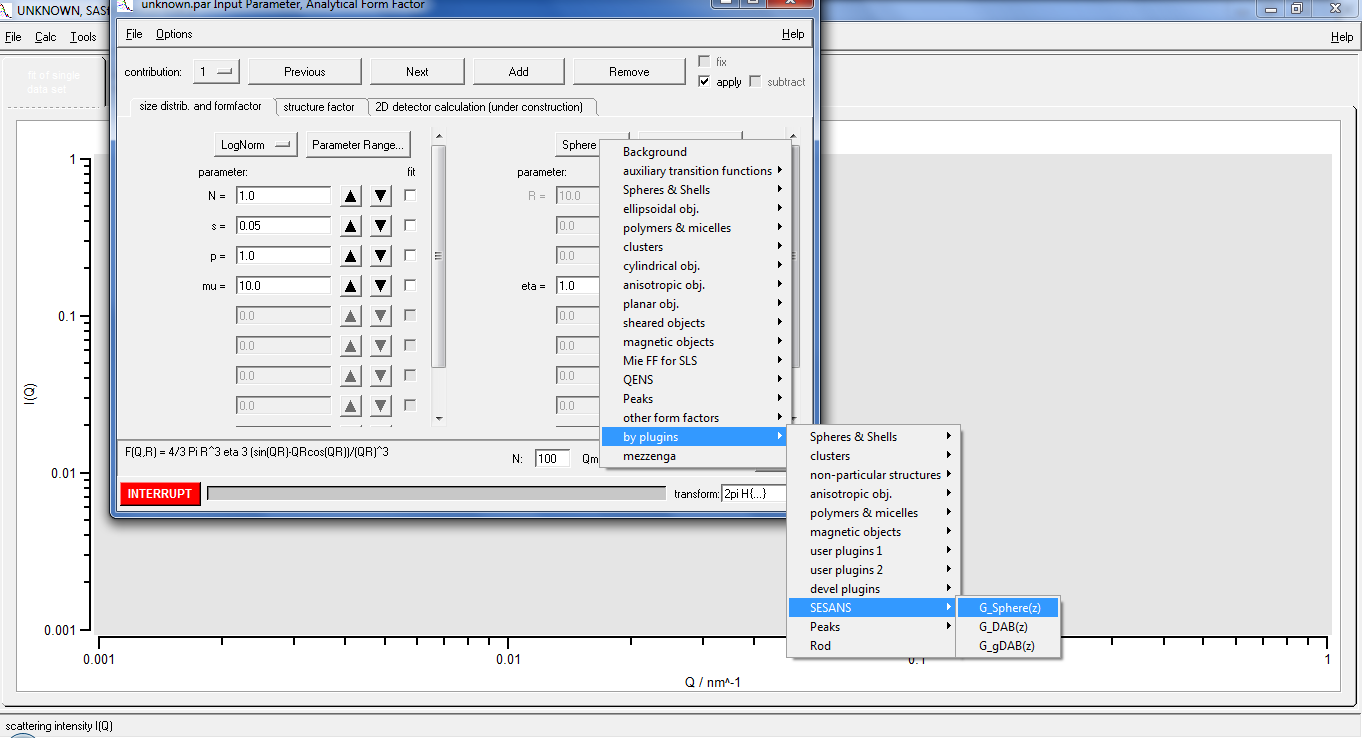
\includegraphics[width=0.7\textwidth]{../images/GUI/GzPlugins.png}
\end{center}
\caption{\SASfit plugins which directly calculate SESANS correlation function}
\label{fig:HankelOp}
\end{figure}

\begin{figure}[htb]
\begin{center}
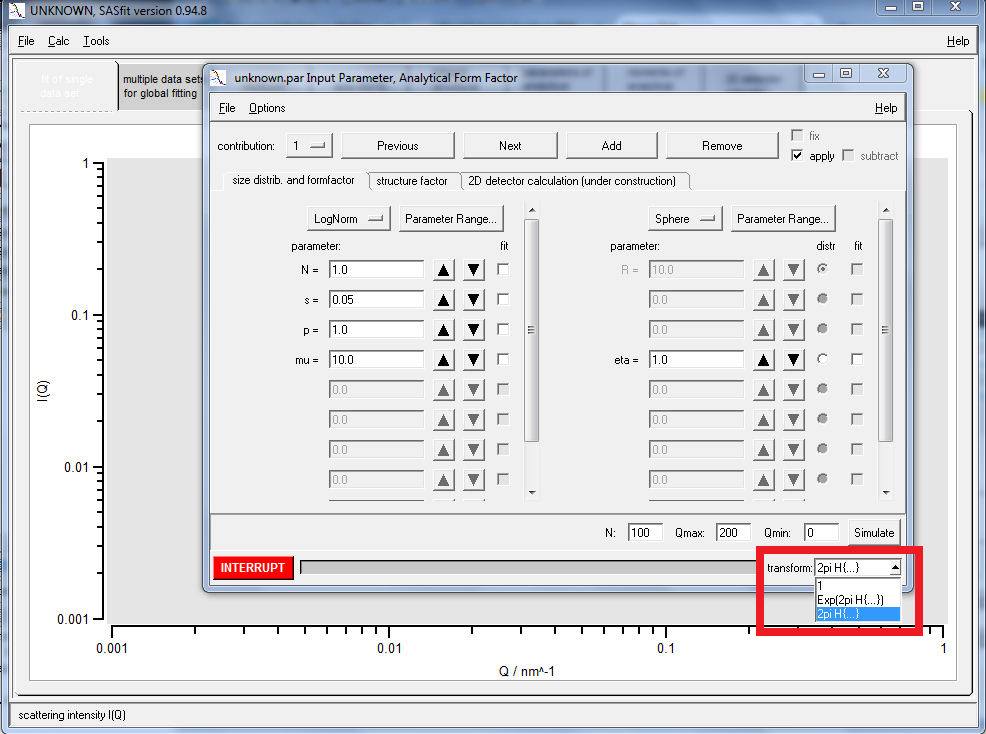
\includegraphics[width=0.7\textwidth]{../images/GUI/HankelOperator.png}
\end{center}
\caption{\SASfit allows to perform a final transformation on the model function to convert a SANS signal into a SESANS signal}
\label{fig:HankelOp}
\end{figure}


\subsection{$G(z)$ of a sphere}
The scattering intensity for a single sphere is given by
\begin{align}
I(Q) &= \left(\frac{4}{3}\pi R^3 \Delta\eta\right)^2 \left(3\frac{\sin QR-QR\cos QR}{Q^3R^3}\right)^2
\end{align}
The unnormalized autocorrelation function for this sphere is given by
\begin{align}
\tilde{\gamma}(r) &=
\begin{cases}
 \Delta\eta^2  \frac{4}{3}\pi R^3 \left( 1-\frac{3}{4}\frac{r}{R}+\frac{1}{16}\left(\frac{r}{R}\right)^3\right) & \mbox{for } r\leq 2R \\
0 & \mbox{for }  r>2R
\end{cases}
\end{align}
and the unnormalized SESANS correlation function
\begin{align}
\tilde{G}_\mathrm{sphere}(z)&= \Delta\eta^2 \pi R^4 \left(\sqrt{1-\xi^2}(2+\xi^2)-\xi^2(\xi^2-4)\ln\left(\frac{\xi}{1+\sqrt{1-\xi^2}}\right)\right)
\end{align}
with $\xi=\frac{z}{2R}$.

\section{$G(z)$ of a randomly distributed, two-phase system (DAB) }~\\
The scattering intensity for a randomly distributed, two-phase system (DAB) is given by
\cite{DebyeBueche1949,DAB1957,Andersson2008}
\begin{align}
I(Q) &= \frac{\left(8 \pi xi^3 \Delta\eta\right)^2}{ \left(1+Q^2\xi^2\right)^2}
\end{align}
The unnormalized autocorrelation function for this sphere is given by
\begin{align}
\tilde{\gamma}(r) &=
 \Delta\eta^2 8\pi\xi^3 \exp\left( -r/\xi\right)
\end{align}
and the unnormalized SESANS correlation function
\begin{align}
\tilde{G}_\mathrm{DAB}(z)&= 8\pi\xi^4 2\frac{z}{\xi}K_1\left(\frac{z}{\xi}\right)
\end{align}

\section{$G(z)$ of a self-affine random density distribution (gDAB) }~\\
The scattering intensity for a randomly distributed, two-phase system (DAB) is given by \cite{Klimes2002,Hunter2006,Andersson2008}
\begin{align}
I(Q) &= \frac{\left(4 \pi \xi^3 (1+2H) \Delta\eta\right)^2}{ \left(1+Q^2\xi^2\right)^{3/2+H}}
\end{align}
The unnormalized autocorrelation function for this sphere is given by
\begin{align}
\tilde{\gamma}(r) &=
 \Delta\eta^2 8a^3\pi\sqrt{\pi}\frac{\Gamma\left(\frac{3}{2}+H\right)}{\Gamma\left(H\right)}\frac{2}{\Gamma(H)}\left(\frac{r}{2a}\right)^H K_H\left(\frac{r}{a}\right)
\end{align}
and the unnormalized SESANS correlation function
\begin{align}
\tilde{G}_\mathrm{gDAB}(z)&=  8a^3\pi\frac{\Gamma\left(\frac{3}{2}+H\right)}{\Gamma^2\left(H\right)} 2\sqrt{az}\left(\frac{z}{2a}\right)^{H+\frac12}K_{\frac12+H}\left(\frac{z}{a}\right)
\end{align} 

\section{$G(z)$ for a generalized Gaussian coil (gGc) }~\\
The scattering intensity for a a generalized Gaussian coil (gGc) has been given by  Hammouda \cite{Hammouda,Hammouda2012,Hammouda1993,Hammouda2016} (see also section \ref{sect:generalized_gaussian_coil}) as
\begin{align}
I_\text{gGc}(q) &= I_0
\left(
\frac{1}{\nu U^{\frac{1}{2 \nu}}} \; \gamma\left(\frac{1}{2 \nu},U\right)-
\frac{1}{\nu U^{\frac{1}{  \nu}}} \; \gamma\left(\frac{1}{  \nu},U\right)
\right)
\label{eq:generalizedGauss1inSESANS}
\end{align}
with the modified variable
\begin{align}
U&= \left(2\nu+1\right)\left(2\nu+2\right)\frac{q^2R_G^2}{6}
\end{align}
and the lower incomplete Gamma Function $\gamma(a,x) = \int_0^x \mathrm{d}t \; t^{a-1} \exp(-t)$.
$\nu$ is the excluded volume parameter from the Flory mean field theory and typical values for them are
\begin{description}
\item[$\nu=1/3$] partially precipitate in poor solvents
\item[$\nu=1/2$] thermally relaxed in "theta"-solvents
\item[$\nu=3/5$] swollen in good solvents
\end{description}
To be able to perform the Hankel transform we start from eq.\ \ref{eq:generalizedGauss} which leads to eq.\ \ref{eq:generalizedGauss1inSESANS}
\begin{align}
P(q) &= 2\int_0^1 \mathrm{d}x \; (1-x)e^{-q^2R_g^2(2\nu+1)(2\nu+2)x^{2\nu}}
\label{eq:generalizedGaussinSESANS}
\end{align}
The unnormalized autocorrelation function the order of integration over $x$ and  over $q$ for the Hankel transform can be changed and one gets
\begin{align}
\tilde{G}_\mathrm{gGc}(z) &=
 I_0 \pi \left(
 \frac{  \left(\frac{3w}{4}\right)^{\frac{1}{2\nu}} \frac{4}{w} \Gamma \left(1-\frac{1}{2 \nu },\frac{3 w}{4}\right)}{\nu  (\nu +1) (2
   \nu +1) R_g^2}-\frac{ \left(\frac{3w}{4}\right)^{\frac{1}{\nu }} \frac{4}{w} \Gamma \left(1-\frac{1}{\nu },\frac{3 w}{4}\right)}{\nu
   (\nu +1) (2 \nu +1) R_g^2} \right)\\
   w &= \frac{z^2}{\left(2 \nu ^2+3 \nu +1\right) R_g^2}
\end{align}
where $\Gamma(a,x) = \int_x^\infty \mathrm{d}t \; t^{a-1} \exp(-t)$ is the upper incomplete Gamma Function.
The limit $\tilde{G}_\mathrm{gGc}(0)$ is only finite for $\nu \in \left(0,\frac12\right)$
\begin{align}
\tilde{G}_\mathrm{gGc}(0) &= I_0 \frac{3 \pi }{\left(4 \nu ^4-5 \nu ^2+1\right) R_g^2} \mbox{~for~} \nu \in \left(0,\frac12\right)
\end{align}